\ofsubsection{Tríade tripla}
%
\ofquote{"Sabia que estávamos destinados a jogar. Vamos começar!"\\}{Quistis}
%
\begin{center} 
\includegraphics[width=\columnwidth]{./art/tripletriad/board.jpg} \end{center}
%
\accf{Tríade tripla} é um jogo de cartas inventado pelo psíquico Orlan, inspirado pelas cartas de tarô.
Primeiro, era jogada por soldados para passar o tempo, mas eventualmente se popularizou entre pessoas de várias idades e profissões.
Antes de iniciar o jogo, cada participante escolhe uma mão de 5 cartas de sua coleção.
O MJ decide quem vai primeiro e ambos os jogadores agem em turnos alternados até que a partida termine.
Durante cada turno, um jogador tem que pôr uma carta num espaço vazio em um tabuleiro de 3x3.
Toda carta tem um número em cada um de seus quatro lados e quando colocada adjacente a uma carta do oponente, os números dos lados que se tocam são comparados. O maior vence e captura a outra carta.
Os jogadores podem somente capturar cartas durante o seu turno, aquela que acabou de ser colocada não pode ser capturada.
Você pode pôr pequenas fichas para acompanhar quem é o atual dono daquela carta. O objetivo é capturar a maioria, aquelas que ainda estão nas suas mãos também contam.
Quando a pontuação final empata, o jogo é reiniciado, até que algum jogador vença.
Mesmo que as regras acima se apliquem, algumas outras extras podem ser usadas por alguns jogadores a depender do local.
Abaixo estão algumas das regras especiais mais comuns.
%
\vfill
%
\oftable{p{0.15\columnwidth} p{0.8\columnwidth}}
{\accf{Regra} & \accf{Descrição}} {
	Aberta &  Ambos os jogadores jogam com a mão à mostra.\ofrow
	Igual & Ao colocar uma carta próxima a outra com o mesmo número em contato, você ainda a captura.\ofrow
	Combo & Ao capturar uma carta, você captura todas as outras adjacentes a ela também, que tenham um número menor do que a dela nos lados que se tocam. A regra é então aplicada a todas as cartas capturadas.\ofrow
	Aleatório & Os jogadores não podem escolher sua mão. Ao invés disso, puxe 5 cartas aleatoriamente.\ofrow
	Morte \newline súbita & No momento de puxar, o jogo é reiniciado e ambos os jogadores usam suas cartas capturadas da partida anterior. 
}
%
\newpage
%
\ofquote{"Posso ver que você coletou e jogou cartas por todo o mundo. Você me lembra dela... seu talento em específico. Ah, já falei demais."\\}{Príncipe de espadas}\\\\
%
Enquanto os torneios da Tríade Tripla geralmente recompensam com Gil, itens ou equipamentos, jogos casuais focam na aquisição de novas cartas.
Com a regra mais comum usada, o vencedor pega uma carta de sua escolha da mão do perdedor.
Contudo, há também regras diferentes para recompensas de cartas, algumas das quais estão listadas abaixo.
Além disso, as cartas também podem ser compradas, vendidas ou trocadas assim como qualquer mercadoria.
Os preços podem variar significativamente a depender da popularidade do jogo e da raridade da carta.
%
\\\\
%
\oftable{p{0.15\columnwidth} p{0.8\columnwidth}}
{\accf{Regra} & \accf{Descrição}} {
    Diferença & O vencedor pega cartas igual à diferença de suas pontuações finais.\ofrow	
    Direta & Ambos os jogadores pegam todas as cartas que estão em sua posse ao final da partida.\ofrow	
	Tudo & Os vencedores pegam todas as 5 cartas da mão do perdedor.
}
%
\vfill
%
%	
\begin{center} 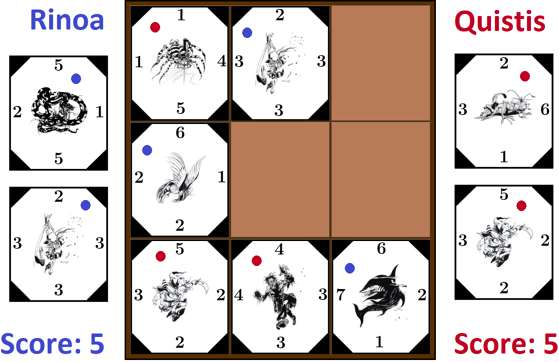
\includegraphics[width=1\columnwidth]{./art/tripletriad/example.jpg} \end{center}
%
No exemplo acima, ambos os jogadores já colocaram 3 cartas e suas pontuações estão empatadas. Os marcadores coloridos nas cartas indicam qual jogador possui cada uma. É a vez de Quistis, então ela também que jogar uma das duas cartas em sua mão em um dos espaços vazios.
Uma jogada forte seria colocar a carta Goblin (aquela de baixo) no espaço central, pois isso permitiria a ela capturar tanto as cartas do centro acima quanto aquelas do centro à esquerda.
Outra jogada esperta seria também colocar qualquer uma delas em um dos outros lugares vazios por segurança, mas isso não a permitiria capturar qualquer uma das cartas de Rinoa. Abaixo está uma lista de cartas de Tríade tripla sorteadas por raridade de cima para baixo.
%At its end, there is a page with backsides, which you can use to print both sides of the cards.
%
\clearpage
%
\newgeometry{bottom=2mm,top=2mm,right=5mm,left=5mm}	
\setlength{\columnsep}{11cm}

\newcommand{\cardback}[0]
{
	
\includegraphics[width=6cm]{./art/tripletriad/cardback.jpg}
	\vskip0.445cm
}

\newcommand{\card}[1]
{
	\includegraphics[width=6cm]{./art/tripletriad/#1.jpg}
	\vskip0.4cm
}
%
\begin{multicols}{3}[][20cm]
%
%col1
\card{l1_astos}
\card{l1_parasite}
\card{l2_helldiver}
\card{l2_worm}
%col2
\card{l1_cobra}
\card{l1_spider}
\card{l2_sahagin}
\card{l3_cockatrice}
%col3
\card{l1_goblin}
\card{l2_bloodsucker}
\card{l2_skeleton}
\card{l3_mantis}
%
\clearpage
%
%col1
\card{l3_nitemare}
\card{l4_eye}
\card{l4_pirate}
\card{l5_ankylo}
%col2
\card{l3_zombie}
\card{l4_gargoyle}
\card{l4_soldier}
\card{l5_deadringer}
%col3
\card{l4_cerberus}
\card{l4_ghost}
\card{l5_adamantoise}
\card{l5_gigas}
%
\clearpage
%
%col1
\card{l5_shark}
\card{l6_medusa}
\card{l7_behemoth}
\card{l7_ochu}
%col2
\card{l6_chimera}
\card{l6_troll}
\card{l7_bull}
\card{l7_witch}
%col3
\card{l6_manticore}
\card{l6_wizard}
\card{l7_giant}
\card{l8_deadrider}
%
\clearpage
%
%col1
\card{l8_ghost}
\card{l9_badman}
\card{l9_vampire}
\card{l10_lich}
%col2
\card{l8_hydra}
\card{l9_dragon}
\card{l10_kraken}
\card{l10_tiamat}
%col3
\card{l8_mancat}
\card{l9_malboro}
\card{l10_marilith}
\card{l10_chaos}
%
\clearpage
%
%\cardback
%\cardback
%\cardback
%\cardback
%\cardback
%\cardback
%\cardback
%\cardback
%\cardback
%\cardback
%\cardback
%\cardback

\end{multicols}

\restoregeometry
\pagebreak